% ---------------------------------------------------------------------------
%  Manuscript prepared for GEOPHYSICS (SEG).
%  Portable build: pdflatex + standard packages (see README.md).
%  To switch to the official SEGTeX class, replace the preamble below with
%  \documentclass[manuscript]{geophysics} and keep the body unchanged.
%  Every number in this manuscript is printed by a cell of
%  ../chapter1_extended.ipynb (sections cited in the comments as [nb Sx]).
% ---------------------------------------------------------------------------
\documentclass[11pt]{article}
\usepackage[margin=1in]{geometry}
\usepackage[T1]{fontenc}
\usepackage{lmodern}
\usepackage{amsmath,amssymb}
\usepackage{graphicx}
\usepackage{booktabs}
\usepackage{siunitx}
\usepackage{setspace}
\usepackage[mathlines]{lineno}
\usepackage[round,authoryear]{natbib}
\usepackage{xcolor}
\usepackage[hidelinks]{hyperref}
\usepackage{caption}
\captionsetup{font=small,labelfont=bf,labelsep=period}
\sisetup{group-minimum-digits=5}

% visible markers for items that require author input before submission
\newcommand{\authornote}[1]{\textcolor{red}{[\textbf{Author note:} #1]}}
\newcommand{\VP}{V_\mathrm{P}}
\newcommand{\VS}{V_\mathrm{S}}
\newcommand{\RPP}{R_\mathrm{PP}}
\newcommand{\Btan}{B_\mathrm{Z}^{\tan}}
\newcommand{\Blsq}{B_\mathrm{Z}^{\mathrm{LSQ}}}
\newcommand{\BAR}{B_\mathrm{AR}}

% notebook-traceability tags: \shownbtrue to display, \shownbfalse for submission
\newif\ifshownb \shownbtrue
\newcommand{\nb}[1]{\ifshownb\textcolor{gray}{[nb #1]}\fi}
\renewcommand{\refname}{REFERENCES}
\doublespacing
\linenumbers

\begin{document}

\begin{center}
{\large\bfseries Error propagation from velocity uncertainty to AVO attribute misclassification:\\
A validated closed-form framework applied to CO$_2$-storage monitoring at Smeaheia}\\[1.5em]
Annaliese J. Lee Seyon$^{1}$ and Abdullatif Alshuhail$^{1}$\\[0.5em]
{\small $^{1}$Department of Geosciences, College of Petroleum Engineering and Geosciences,\\
King Fahd University of Petroleum and Minerals (KFUPM), Dhahran, Saudi Arabia}\\[0.5em]
\authornote{confirm both affiliations; add the corresponding author and e-mail}\\[1em]
\textit{Running head:} Velocity errors and AVO misclassification
\end{center}

% ===========================================================================
\section*{ABSTRACT}
% 246 words (GEOPHYSICS limit: 250)
Amplitude-variation-with-offset (AVO) classification of the top of a CO$_2$-charged reservoir depends on the P-wave velocities assigned to the caprock and the reservoir. We derive closed-form sensitivities of the two-term Shuey intercept $A$ and gradient $B$ to relative P-velocity errors, including the dependence of Poisson's ratio on $\VP$. We validate the symbolic implementation against an independent derivation and apply it to a Draupne shale over CO$_2$-saturated Sognefjord sand model of the Smeaheia storage site, northern North Sea. The baseline response is Class III ($A_0=-0.214$, $B_0=-0.021$). The intercept stays negative for all errors within $\pm10\%$, but the gradient is close to zero and highly sensitive. Two-term Shuey reflectivity predicts an apparent Class III$\to$IV transition at a minimum error-vector magnitude of 4.44\%. We recompute this threshold with exact Zoeppritz reflectivity, implemented twice and validated to $2\times10^{-15}$ against a closed-form solution, energy conservation, and two open-source libraries. The exact normal-incidence gradient raises the threshold to 5.58\%, and a two-term least-squares fit over 0\textdegree--30\textdegree{} raises it to 8.23\%. Two-term Shuey therefore understates the error needed for misclassification by about 20\%, but the misclassification itself is physical. Common-mode velocity errors do not cancel in $B$: with Poisson's ratio treated as a function of $\VP$, the first-order caprock sensitivity changes sign. Published seismic-to-well $\VP$ prediction errors in the Smeaheia reservoir interval are 13\%--17\% of the mean log velocity. At that level, AVO class assignment at this interface should be regarded as uncertain unless the elastic model is independently constrained.

% ===========================================================================
\section*{INTRODUCTION}

Amplitude variation with offset (AVO) is routinely used to infer pore-fluid content from the angle dependence of P-wave reflectivity \citep{rutherford1989,castagna1993,castagna1998}. The intercept--gradient crossplot and the classification of \citet{rutherford1989}, extended by \citet{castagna1998}, give the interpreter a compact vocabulary. A Class III response (negative intercept, negative gradient; brightening with offset) is the classical signature of a low-impedance gas or CO$_2$ sand beneath shale. A Class IV response (negative intercept, positive gradient; dimming with offset) arises when a soft sand is capped by a lithology of relatively high S-wave velocity, so that the S-wave contrast reverses the sign of the gradient \citep{castagna1998}.

Amplitude-preserving processing aims to retain relative amplitudes with angle, but quantitative interpretation still rests on an elastic model. That model is used to build fluid-substitution templates, to forward-model expected responses, and to decide whether an observed anomaly is consistent with CO$_2$. The P-wave velocities of the model are among its least certain inputs. They come from sonic logs that may not represent the seismic-scale interval, from seismic inversion, or from machine-learning property prediction. At the Smeaheia CO$_2$-storage prospect, the published multi-attribute-regression and probabilistic-neural-network predictions of $\VP$ have validation RMS errors of \SI{380.91}{m/s} and \SI{461.3}{m/s}, respectively \citep[][their Table 12]{hema2027}. Relative to the mean Sognefjord log velocities in wells 32/4-1 and 32/2-1, these errors equal 12.80\%--16.95\% \nb{\S9.7}.

For CO$_2$-storage monitoring, a velocity-induced change of AVO class has a direct interpretational cost. If velocity errors turn a genuine Class III CO$_2$ response into an apparent Class IV, the interpreter may reject a correct CO$_2$ interpretation or misplace a plume boundary. The concern is sharpened at Smeaheia because the brine-sand reference response lies close to $B=0$ (this study), so fluid discrimination relies on small gradient differences.

This paper asks a narrow, quantitative question: how large must relative errors in the caprock and reservoir P-velocities be before the AVO class of the Smeaheia top reservoir changes, and how much of the answer depends on the reflectivity approximation used? We make four contributions:
\begin{enumerate}
\item a closed-form sensitivity analysis of the \citet{shuey1985} intercept and gradient to layer $\VP$ errors, cross-validated against an independent symbolic derivation;
\item the total (chain-rule) sensitivity of the gradient when Poisson's ratio is treated as a function of $\VP$, and a demonstration that the fixed-Poisson's-ratio sensitivity is misleading;
\item a machine-precision exact-Zoeppritz \citep{zoeppritz1919} recomputation of the class-change threshold, which separates approximation artifacts from physical effects;
\item a quantification of how strongly the threshold depends on the angle aperture used to estimate the gradient.
\end{enumerate}

% ===========================================================================
\section*{THEORY AND METHOD}

\subsection*{Elastic model}

The reference model (Table~\ref{tab:model}) represents the Draupne Formation shale caprock over Sognefjord Formation sandstone at approximately \SI{1200}{m} true vertical depth subsea in the Smeaheia area \citep{fawad2021a,fawad2021b,hema2027}. The CO$_2$-sand properties were obtained by \citet{gassmann1951} fluid substitution of the brine-sand model \authornote{specify the CO$_2$ equation of state or property source, saturation model, and the pressure and temperature used; the source notebook gives $S_{\mathrm{CO_2}}\approx0.6$, $T\approx\SI{40}{\celsius}$, $P_\mathrm{pore}\approx\SI{11}{MPa}$}. We treat the model as fixed input. As a consistency check, Gassmann's relations leave the shear modulus unchanged, which predicts $\VS^{\mathrm{CO_2}}=\VS^{\mathrm{brine}}(\rho^{\mathrm{brine}}/\rho^{\mathrm{CO_2}})^{1/2}=\SI{1183.5}{m/s}$, compared with the model value of \SI{1180}{m/s} \nb{\S9.7}.

\begin{table}[htbp]
\centering
\caption{Reference elastic model (fixed input). Subscript 1 denotes the caprock and subscript 2 the reservoir.}
\label{tab:model}
\begin{tabular}{lccc}
\toprule
Property & Caprock (Draupne shale) & Brine sand & CO$_2$ sand \\
\midrule
$\VP$ (m/s) & 2600 & 2200 & 1950 \\
$\VS$ (m/s) & 1200 & 1150 & 1180 \\
$\rho$ (kg/m$^3$) & 2350 & 2150 & 2030 \\
Poisson's ratio $\sigma$ & 0.3647 & -- & 0.2111 \\
\bottomrule
\end{tabular}
\end{table}

The active scenario, shale over CO$_2$ sand, has contrasts $\Delta\VP/\bar V_\mathrm{P}=-0.2857$, $\Delta\VS/\bar V_\mathrm{S}=-0.0168$, and $\Delta\rho/\bar\rho=-0.1461$ \nb{\S9.2}. These contrasts are not small, so the accuracy of weak-contrast reflectivity cannot be taken for granted.

\subsection*{Two-term Shuey attributes}

Following \citet{shuey1985} in the form given by \citet{castagna1993} and \citet{wiggins1983}, the intercept, the P-velocity contrast, and the gradient are
\begin{equation}
A=\frac{\rho_2V_{\mathrm{P}2}-\rho_1V_{\mathrm{P}1}}{\rho_2V_{\mathrm{P}2}+\rho_1V_{\mathrm{P}1}},\qquad
C=\frac{V_{\mathrm{P}2}-V_{\mathrm{P}1}}{V_{\mathrm{P}2}+V_{\mathrm{P}1}},
\label{eq:A}
\end{equation}
\begin{equation}
B=A\left[D-\frac{2(1+D)(1-2\bar\sigma)}{1-\bar\sigma}\right]+\frac{\Delta\sigma}{(1-\bar\sigma)^2},\qquad
D=\left[1+\frac{(\rho_2-\rho_1)/(\rho_2+\rho_1)}{(V_{\mathrm{P}2}-V_{\mathrm{P}1})/(V_{\mathrm{P}2}+V_{\mathrm{P}1})}\right]^{-1},
\label{eq:B}
\end{equation}
where $\bar\sigma=(\sigma_1+\sigma_2)/2$, $\Delta\sigma=\sigma_2-\sigma_1$, and
\begin{equation}
\sigma_i=\frac{V_{\mathrm{P}i}^2-2V_{\mathrm{S}i}^2}{2\left(V_{\mathrm{P}i}^2-V_{\mathrm{S}i}^2\right)}.
\label{eq:sigma}
\end{equation}
The intercept in equation~\ref{eq:A} is the exact normal-incidence plane-wave reflection coefficient; our Zoeppritz implementation reproduces it to $5.6\times10^{-17}$ \nb{\S9.1}. We classify responses with $A<0$ as Class III when $B<0$ and as Class IV when $B>0$ \citep{castagna1998}. The class-change boundary studied here is therefore $B=0$.

\subsection*{Linear error propagation}

Let $r_i=\delta V_{\mathrm{P}i}/V_{\mathrm{P}i}$ be the relative P-velocity error in layer $i$. Because $A$ and $C$ depend on $\VP$ only through the ratio $V_{\mathrm{P}2}/V_{\mathrm{P}1}$, their first-order relative errors take the form
\begin{equation}
\frac{\delta X}{X}=k_X\,(r_1-r_2),\qquad X\in\{A,C\},
\label{eq:kX}
\end{equation}
so errors common to both layers (common-mode errors) cancel exactly. The same form holds for $B$ \emph{only} if $\bar\sigma$ and $\Delta\sigma$ are held fixed during differentiation. We call the corresponding coefficient $k_B$ the fixed-$\sigma$ sensitivity. Physically, $\sigma_i$ depends on $V_{\mathrm{P}i}$ through equation~\ref{eq:sigma}. The total sensitivity is then
\begin{equation}
\frac{\mathrm{d}B}{\mathrm{d}\ln V_{\mathrm{P}i}}=\left.\frac{\partial B}{\partial\ln V_{\mathrm{P}i}}\right|_{\sigma}+\frac{\partial B}{\partial\sigma_i}\,\frac{\partial\sigma_i}{\partial\ln V_{\mathrm{P}i}},\qquad
\frac{\partial\sigma_i}{\partial\ln V_{\mathrm{P}i}}=\frac{V_{\mathrm{P}i}^2V_{\mathrm{S}i}^2}{\left(V_{\mathrm{P}i}^2-V_{\mathrm{S}i}^2\right)^2},
\label{eq:total}
\end{equation}
which is derived in Appendix~B. The second term is not antisymmetric in the two layers. As a result, common-mode errors do not cancel in $B$.

\subsection*{Nonlinear error mapping}

To go beyond first order, we re-evaluate equations~\ref{eq:A}--\ref{eq:sigma} exactly at perturbed velocities, recomputing $\sigma$ at each perturbed $\VP$ and leaving $\VS$ and $\rho$ unperturbed. We use (1) one-dimensional slices (caprock only, reservoir only, and $r_2=-r_1$), (2) the full error plane $(r_1,r_2)\in[-10\%,10\%]^2$, and (3) radial spokes $r_1=|r|\cos\phi$, $r_2=|r|\sin\phi$ with $|r|\le10\%$. Along each spoke we locate $B=0$ by bracketed root finding (Brent's method, tolerance $10^{-12}$). The minimum-radius threshold is then found by bounded minimisation over $\phi$.

\subsection*{Exact Zoeppritz reflectivity and gradient estimators}

We implemented the exact plane-wave P--P reflection coefficient twice, independently:
\begin{itemize}
\item by solving the $4\times4$ Zoeppritz system for $[\RPP,R_\mathrm{PS},T_\mathrm{PP},T_\mathrm{PS}]$ at each angle;
\item by the explicit closed form of \citet[][their equation 5.39]{aki1980} (Appendix~A), written in vertical slownesses with a complex square-root branch so that it remains valid beyond critical angles.
\end{itemize}
An exact gradient is not uniquely defined, because exact $\RPP$ is not linear in $\sin^2\theta$. We therefore use two definitions:
\begin{itemize}
\item the \emph{exact tangent gradient}, $\Btan=\partial\RPP/\partial(\sin^2\theta)|_{\theta=0}$, obtained from a degree-6 least-squares polynomial in $\sin^2\theta$ fitted to exact $\RPP$ on 0\textdegree--20\textdegree. This is the exact counterpart of the Shuey gradient, which is also a normal-incidence slope. Between polynomial degrees 6 and 10 it changes by $1.0\times10^{-9}$ \nb{\S9.2};
\item the \emph{two-term least-squares gradient}, $\Blsq$: the slope of $\RPP\approx A+B\sin^2\theta$ fitted to exact $\RPP$ on 0\textdegree--30\textdegree. This is the gradient that a two-term AVO inversion of noise-free, ideally processed gathers would recover.
\end{itemize}
We also evaluate the linearised gradient of \citet{aki1980},
\begin{equation}
\BAR=\frac12\frac{\Delta\VP}{\bar V_\mathrm{P}}-2\left(\frac{\bar V_\mathrm{S}}{\bar V_\mathrm{P}}\right)^2\left(\frac{\Delta\rho}{\bar\rho}+2\frac{\Delta\VS}{\bar V_\mathrm{S}}\right),
\label{eq:BAR}
\end{equation}
of which Shuey's expression is a re-parameterisation that agrees to first order in the contrasts. Approximations that retain terms quadratic in the elastic contrasts also exist \citep{wang1999}; we do not use them here, because the exact solution is available at negligible cost.

\subsection*{Verification}

The symbolic engine (SymPy) was checked against an independent Mathematica derivation using that derivation's own test model. The Python implementation reproduces all six reference outputs to the printed precision (Table~\ref{tab:mma}) \nb{\S2.1}.

\begin{table}[htbp]
\centering
\caption{Cross-validation of the symbolic engine against an independent Mathematica derivation. Test model: $V_{\mathrm{P}1}=\SI{3599}{m/s}$, $V_{\mathrm{P}2}=\SI{3930}{m/s}$, $V_{\mathrm{S}1}=\SI{2341.45}{m/s}$, $V_{\mathrm{S}2}=\SI{2304.5}{m/s}$, $\rho_1=\SI{2313.9}{kg/m^3}$, $\rho_2=\SI{2388.72}{kg/m^3}$.}
\label{tab:mma}
\begin{tabular}{lrr}
\toprule
Quantity & Python (SymPy) & Mathematica \\
\midrule
$A$   & $+0.059832$ & $+0.0598318$ \\
$B$   & $+0.041834$ & $+0.0418341$ \\
$C$   & $+0.043963$ & $+0.0439633$ \\
$k_A$ & $-8.32684827$ & $-8.32685$ \\
$k_B$ (fixed $\sigma$) & $+24.87862148$ & $+24.8786$ \\
$k_C$ & $-11.35113011$ & $-11.3511$ \\
\bottomrule
\end{tabular}
\end{table}

Both Zoeppritz implementations were required to agree to better than $10^{-13}$ before either was used. We tested four models on 0\textdegree--60\textdegree: the two Smeaheia scenarios, the Mathematica test model, and a model with a P-wave critical angle of 41.8\textdegree. The maximum discrepancies are listed in Table~\ref{tab:zoep} \nb{\S9.1}. Finally, all three normal-incidence gradients converge to $\Btan$ as the contrasts vanish, with relative deviation proportional to the contrast. For contrast parameters of $10^{-1}$, $10^{-2}$, and $10^{-3}$ the deviation is $9.5\times10^{-2}$, $1.3\times10^{-2}$, and $1.4\times10^{-3}$ for $\BAR$, and $6.9\times10^{-2}$, $1.3\times10^{-2}$, and $1.4\times10^{-3}$ for the Shuey gradient \nb{\S9.2}.

\begin{table}[htbp]
\centering
\caption{Verification of the exact Zoeppritz implementations (maximum absolute discrepancy over four models and 121 angles on 0\textdegree--60\textdegree).}
\label{tab:zoep}
\begin{tabular}{lr}
\toprule
Check & Maximum discrepancy \\
\midrule
$4\times4$ matrix solution vs.\ explicit \citet{aki1980} form & $1.86\times10^{-15}$ \\
$\RPP(0)$ vs.\ $(Z_2-Z_1)/(Z_2+Z_1)$ & $1.73\times10^{-16}$ \\
Energy-flux conservation, $|\sum E-1|$ & $7.77\times10^{-16}$ \\
PyLops \texttt{zoeppritz\_pp} (pre-critical angles) & $5.41\times10^{-16}$ \\
bruges \texttt{zoeppritz\_rpp} (conjugated post-critically$^{a}$) & $1.26\times10^{-15}$ \\
\bottomrule
\multicolumn{2}{l}{\footnotesize $^{a}$bruges uses the opposite Fourier sign convention; PyLops returns NaN beyond a critical angle.}
\end{tabular}
\end{table}

% ===========================================================================
\section*{RESULTS}

\subsection*{Baseline response and linear sensitivities}

The shale over CO$_2$-sand baseline gives $A_0=-0.2137$, $B_0=-0.0211$, and $C_0=-0.1429$, a Class III response. The shale over brine-sand reference gives $A_0=-0.1273$ and $B_0=+0.0023$ \nb{\S3}. With $A<0$ and $B>0$, the brine reference therefore falls marginally within the Class IV quadrant. The linear coefficients at the CO$_2$ baseline are $k_A=+2.233$, $k_B=-31.277$ (fixed $\sigma$), and $k_C=+3.429$ \nb{\S3}. The large relative sensitivity of $B$ is mainly a consequence of the small baseline gradient. The absolute fixed-$\sigma$ sensitivity $\partial B/\partial\ln V_{\mathrm{P}1}=+0.660$ is unremarkable, but it is divided by $|B_0|=0.021$ \nb{\S9.6}.

\subsection*{Nonlinear response over the error plane}

The intercept is nearly linear in the velocity errors and remains negative over the entire $\pm10\%$ error plane, with a maximum of $A=-0.116$ (Figure~\ref{fig:slices}a) \nb{\S9.8}. The stack-amplitude bright spot is therefore robust to these errors. The gradient, in contrast, is strongly nonlinear (Figure~\ref{fig:slices}b). The product $A\cdot B$, which is $+0.00451$ at the baseline, ranges from $-0.00676$ to $+0.01444$ over the error plane and changes sign across the $B=0$ contour (Figure~\ref{fig:gi}) \nb{\S5}.

\begin{figure}[htbp]
\centering
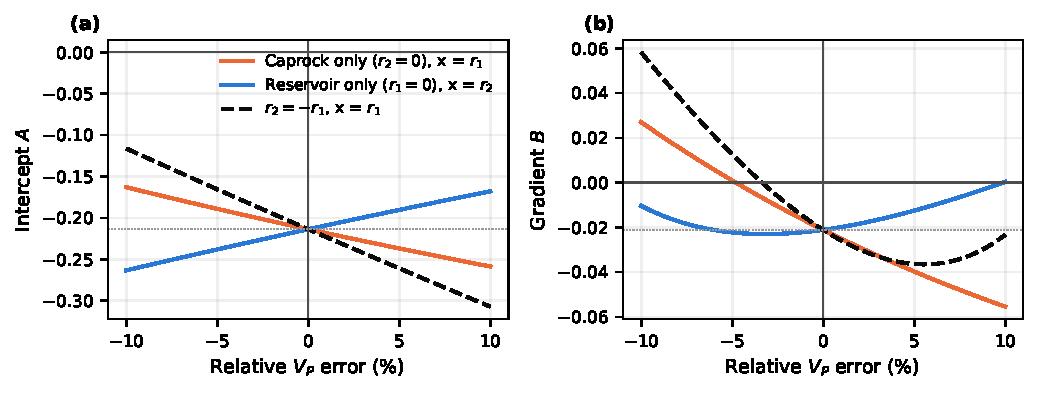
\includegraphics[width=\textwidth]{figures/fig01_AB_slices.pdf}
\caption{(a) Intercept $A$ and (b) two-term Shuey gradient $B$ versus relative $\VP$ error for caprock-only ($r_2=0$), reservoir-only ($r_1=0$), and $r_2=-r_1$ perturbations. Shale over CO$_2$ sand; $\sigma$ is recomputed at each perturbed velocity. Dotted lines mark the baseline values.}
\label{fig:slices}
\end{figure}

\begin{figure}[htbp]
\centering
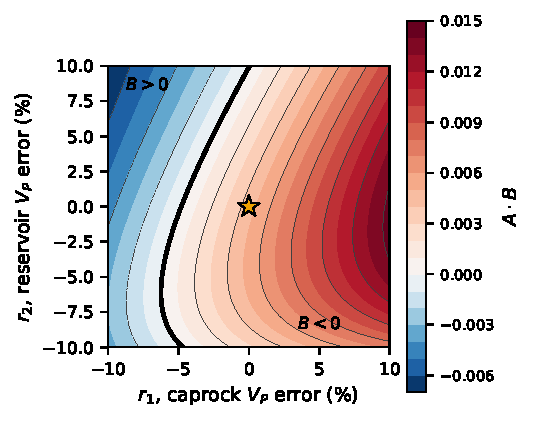
\includegraphics[width=0.55\textwidth]{figures/fig02_GI_map.pdf}
\caption{Product $A\cdot B$ over the $(r_1,r_2)$ error plane (two-term Shuey). The thick black line is $B=0$, the apparent Class III/IV boundary; the star marks the baseline. The colour scale is diverging about zero.}
\label{fig:gi}
\end{figure}

Figure~\ref{fig:spokes} shows the migration of the response in the crossplot. At $|r|=10\%$ the Shuey gradient ranges from $-0.0554$ (caprock-only positive error, $\phi=0^\circ$) to $+0.0304$ ($\phi=135^\circ$, caprock slow and reservoir fast) \nb{\S9.3}. With two-term Shuey, $B=0$ is crossed at $|r|=4.752\%$ along $\phi=135^\circ$, which corresponds to $r_1-r_2=-6.721\%$. The closest approach of the boundary to the baseline is $|r|=4.444\%$ at $\phi=156.6^\circ$, that is, $r_1=-4.079\%$ and $r_2=+1.765\%$ \nb{\S9.3}. The common-mode spokes ($\phi=45^\circ$, $225^\circ$) are not short. The $\phi=225^\circ$ spoke reaches $B=+0.0033$ at $|r|=10\%$ \nb{\S9.3}, a first indication that common-mode errors do not cancel in $B$.

\begin{figure}[htbp]
\centering
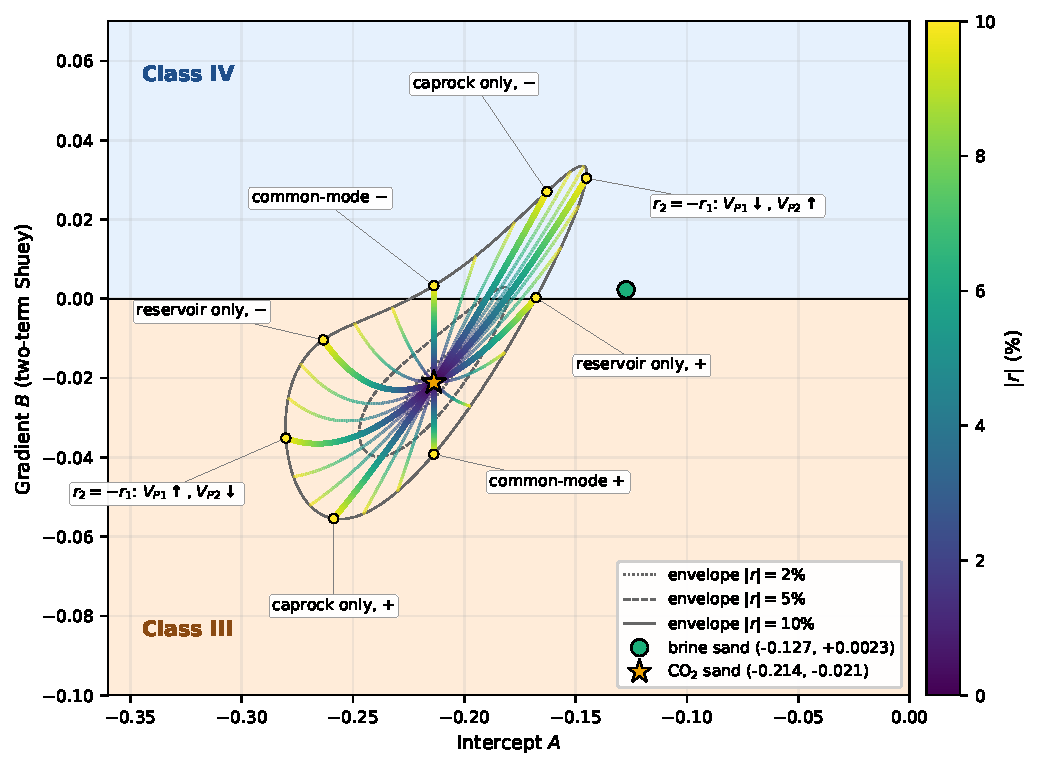
\includegraphics[width=\textwidth]{figures/fig03_AB_spokes.pdf}
\caption{Radial error spokes in the $A$--$B$ crossplot (two-term Shuey), coloured by error magnitude $|r|$, for 24 error directions $\phi$ in the $(r_1,r_2)$ plane; the eight labelled spokes are the cardinal and diagonal directions. Envelopes are shown at $|r|=2\%$, 5\%, and 10\%. The brine-sand reference is shown for comparison.}
\label{fig:spokes}
\end{figure}

\subsection*{Exact Zoeppritz versus two-term Shuey}

At the baseline the gradient estimators differ substantially (Figure~\ref{fig:rpp}, Table~\ref{tab:thr}) \nb{\S9.2}. The two-term Shuey gradient ($-0.0211$) is 0.705 times the exact tangent gradient ($-0.0299$), that is, about 30\% closer to the class boundary. The Aki--Richards gradient ($-0.0445$) errs in the opposite direction. The 0\textdegree--30\textdegree{} least-squares gradient ($-0.0513$) is steeper than the tangent, because exact $\RPP$ curves downward in $\sin^2\theta$ at this interface (Figure~\ref{fig:rpp}).

\begin{figure}[htbp]
\centering
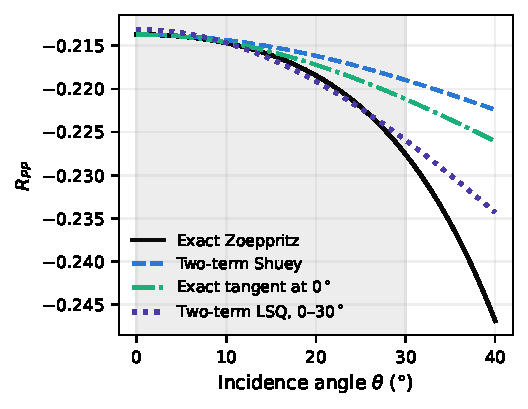
\includegraphics[width=0.55\textwidth]{figures/fig04_rpp_baseline.pdf}
\caption{Exact Zoeppritz $\RPP(\theta)$ at the baseline (shale over CO$_2$ sand) compared with the two-term Shuey curve, the exact normal-incidence tangent, and the two-term least-squares fit over 0\textdegree--30\textdegree{} (shaded).}
\label{fig:rpp}
\end{figure}

\begin{table}[htbp]
\centering
\caption{Baseline gradient and $B=0$ threshold $|r|$ (\%) by gradient estimator, along selected error directions $\phi$ and at the closest approach to the baseline; ``--'' denotes no crossing within $|r|\le10\%$. No estimator crosses $B=0$ along $\phi=0^\circ$, $45^\circ$, $270^\circ$, or $315^\circ$. The last column is the fraction of the $\pm10\%$ error square in which $B>0$ \nb{\S9.2, \S9.4, \S9.5}.}
\label{tab:thr}
\small
\begin{tabular}{lrrrrrrr}
\toprule
Estimator & $B_0$ & $\phi=90^\circ$ & $\phi=135^\circ$ & $\phi=180^\circ$ & $\phi=225^\circ$ & Min.\ $|r|$ ($\phi$) & $B>0$ \\
\midrule
Two-term Shuey          & $-0.0211$ & 9.900 & 4.752 & 4.802 & 8.826 & 4.444 (156.6\textdegree) & 29.55\% \\
Aki--Richards           & $-0.0445$ & --    & 6.206 & 7.064 & --    & 6.035 (148.5\textdegree) & 16.95\% \\
Zoeppritz, tangent      & $-0.0299$ & --    & 5.755 & 6.484 & --    & 5.580 (149.2\textdegree) & 19.05\% \\
Zoeppritz, LSQ 0--30\textdegree & $-0.0513$ & -- & 8.455 & 9.628 & -- & 8.225 (148.5\textdegree) & 8.75\% \\
\bottomrule
\end{tabular}
\end{table}

Three results follow (Figure~\ref{fig:b0}):
\begin{enumerate}
\item \textbf{The misclassification is physical.} Every exact-reflectivity estimator predicts a Class III$\to$IV transition within $\pm10\%$ when the caprock velocity is underestimated relative to the reservoir velocity.
\item \textbf{Two-term Shuey places the threshold too low.} Along $\phi=135^\circ$ the exact tangent threshold is 5.755\% versus 4.752\% for Shuey, a shortfall of 1.003 percentage points, or 17.4\% of the exact value. At the closest-approach point the thresholds are 5.580\% versus 4.444\%, a shortfall of 1.136 points, or 20.4\% \nb{\S9.4}. The bias comes mainly from the baseline gradient, which Shuey places too close to zero.
\item \textbf{Some Shuey crossings are artifacts.} Two-term Shuey predicts crossings for reservoir-only errors ($\phi=90^\circ$, at 9.900\%) and for common-mode errors ($\phi=225^\circ$, at 8.826\%). No exact estimator reproduces either crossing.
\end{enumerate}

\begin{figure}[htbp]
\centering
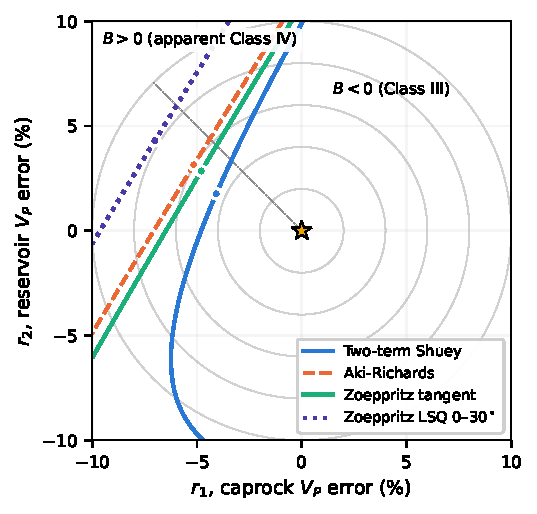
\includegraphics[width=0.55\textwidth]{figures/fig05_B0_contours.pdf}
\caption{Class III/IV boundary ($B=0$) in the $(r_1,r_2)$ error plane for two-term Shuey, Aki--Richards, the exact Zoeppritz tangent, and the 0\textdegree--30\textdegree{} least-squares Zoeppritz gradient. Dots mark each boundary's closest approach to the baseline (star); the dash-dotted line is the $\phi=135^\circ$ spoke; grey circles are $|r|=2\%$--10\%.}
\label{fig:b0}
\end{figure}

\subsection*{Dependence on the angle aperture}

When $B$ is estimated by a two-term fit to exact reflectivity, both the baseline gradient and the threshold depend on the aperture (Table~\ref{tab:aperture}) \nb{\S9.4}. The threshold along $\phi=135^\circ$ rises from 6.993\% for a 0\textdegree--20\textdegree{} fit to 9.355\% for 0\textdegree--35\textdegree. With a 0\textdegree--40\textdegree{} fit, no crossing occurs within $\pm10\%$.

\begin{table}[htbp]
\centering
\caption{Aperture dependence of the two-term least-squares gradient fitted to exact Zoeppritz reflectivity \nb{\S9.4}.}
\label{tab:aperture}
\begin{tabular}{lrr}
\toprule
Aperture & $B_0$ (LSQ) & Threshold along $\phi=135^\circ$ \\
\midrule
0\textdegree--20\textdegree & $-0.0389$ & 6.993\% \\
0\textdegree--25\textdegree & $-0.0443$ & 7.662\% \\
0\textdegree--30\textdegree & $-0.0513$ & 8.455\% \\
0\textdegree--35\textdegree & $-0.0601$ & 9.355\% \\
0\textdegree--40\textdegree & $-0.0711$ & -- \\
\bottomrule
\end{tabular}
\end{table}

\subsection*{Poisson's ratio and the failure of common-mode cancellation}

Evaluating equation~\ref{eq:total} at the baseline gives the following \nb{\S9.6, \S10.1}:
\begin{itemize}
\item \emph{Fixed $\sigma$}: $\partial B/\partial\ln V_{\mathrm{P}1}=+0.6603$ and $\partial B/\partial\ln V_{\mathrm{P}2}=-0.6603$. The sum is zero, so common-mode errors cancel.
\item \emph{Total}: $\mathrm{d}B/\mathrm{d}\ln V_{\mathrm{P}1}=-0.4050$ and $\mathrm{d}B/\mathrm{d}\ln V_{\mathrm{P}2}=+0.1114$. The sum is $-0.2936$, so common-mode errors do not cancel.
\end{itemize}
The chain-rule factors are $\partial B/\partial\sigma_1=-3.0974$ and $\partial B/\partial\sigma_2=+0.8467$, with $\partial\sigma_1/\partial\ln V_{\mathrm{P}1}=0.3439$ and $\partial\sigma_2/\partial\ln V_{\mathrm{P}2}=0.9115$. The caprock sensitivity therefore changes sign.

To first order along $\phi=135^\circ$, the fixed-$\sigma$ sensitivity predicts that $B$ becomes more negative, with no crossing at all. The total sensitivity predicts a crossing at 5.782\%, against 4.752\% from the full nonlinear Shuey evaluation \nb{\S9.6}.

Common-mode errors of $\pm10\%$ also move $B$ when it is computed from exact reflectivity. The exact tangent gradient changes from $-0.0299$ to $-0.0433$ ($+10\%$) and to $-0.0117$ ($-10\%$), while $A$ is exactly invariant \nb{\S9.6}. The reason is that exact $\RPP$ depends only on velocity ratios and density ratios. Scaling $\VP$ in both layers while holding $\VS$ fixed changes $\VS/\VP$, and hence $\sigma$, in each layer.

% ===========================================================================
\section*{DISCUSSION}

\subsection*{What exact reflectivity changes}

The conclusion drawn from two-term Shuey reflectivity survives exact reflectivity: differential $\VP$ errors of a few percent can change the apparent AVO class at the Smeaheia top reservoir. Its magnitude does not survive unchanged. At the contrasts of this interface ($\Delta\VP/\bar V_\mathrm{P}\approx-0.29$), terms of second order in the contrasts are not negligible. The two first-order parameterisations, Shuey and Aki--Richards, bracket the exact tangent gradient from opposite sides (Table~\ref{tab:thr}). Two-term Shuey therefore overstates the vulnerability of the classification by 17\%--20\% in required error magnitude, and it produces spurious crossings for reservoir-only and common-mode errors. We did not decompose the Shuey--Aki--Richards difference into individual second-order terms. The attribution to second-order contrast terms rests on the small-contrast convergence test, not on an explicit expansion. The quadratic-in-contrast expressions of \citet{wang1999} would allow such a decomposition.

\subsection*{Which gradient should define the class?}

The tangent gradient is the correct reference for judging the Shuey formula itself. A two-term inversion of recorded gathers, however, returns an aperture-dependent slope. For this interface that slope is steeper than the tangent, so the practical threshold moves to 7.0\%--9.4\% for apertures of 20\textdegree--35\textdegree, and beyond 10\% for a 40\textdegree{} aperture (Table~\ref{tab:aperture}). A class label obtained from a two-term fit is therefore partly a property of the acquisition aperture and not only of the rocks. Where $B$ is close to zero, we recommend reporting the aperture together with any AVO class assignment.

\subsection*{Is a $\pm10\%$ velocity error realistic?}

The Smeaheia seismic-to-well $\VP$ predictions of \citet{hema2027} have validation RMS errors of 12.80\%--16.95\% of the mean Sognefjord log velocity \nb{\S9.7}. These are errors of a property-prediction workflow, not of processing velocities, and they refer to the reservoir interval rather than to the caprock--reservoir differential. They nevertheless indicate that $\VP$ uncertainties from several percent up to more than 10\% are plausible for elastic models built at Smeaheia. At that level, the exact minimum thresholds of 5.6\%--8.2\% lie within the uncertainty.

\subsection*{Scope and limitations}

The framework propagates errors in the layer P-velocities that enter the reflection coefficient, that is, errors in the elastic model used for interpretation. Processing-velocity errors act mainly through a different mechanism, the incidence angle assigned to each offset, which is not modelled here. Density and $\VS$ errors are also not propagated. Because $\sigma$ depends on $\VS$ as well as $\VP$, a $\VS$ error would interact with the effects described above.

The analysis further assumes isotropic, elastic, planar interfaces and a single interface without tuning, with noise-free reflectivity. Anisotropy, attenuation, thin-bed interference, and angle-dependent wavelet effects can all modify the observed gradient.

\subsection*{Model calibration}

The brine-sand $\VP$ of the reference model (\SI{2200}{m/s}) is 19.2\% and 26.1\% below the mean Sognefjord log velocities in wells 32/2-1 and 32/4-1. It is also below the minimum log value in both wells, which is \SI{2436}{m/s} in 32/2-1 and \SI{2748}{m/s} in 32/4-1 \citep[][their Tables 1 and 2]{hema2027} \nb{\S9.7}. The CO$_2$-sand model inherits this offset. The absolute values of $A$, $B$, and the thresholds reported here should therefore be read as representative of a soft-sand end member, not as calibrated Smeaheia values. The methodology and the relative conclusions (Shuey versus Zoeppritz, and the role of $\sigma$) do not depend on this calibration; the numerical thresholds do.

\authornote{Either justify the soft-sand end member (for example, from a seismic-scale or upscaled velocity at the injection point) or recalibrate the model to the well data and re-run the notebook before submission.}

% ===========================================================================
\section*{CONCLUSIONS}

A symbolic implementation of the Shuey intercept and gradient, cross-validated against an independent derivation, shows that the Class III baseline of the Smeaheia top reservoir has a robust intercept but a gradient close to zero. A Class III$\to$IV misclassification is physically possible within $\pm10\%$ P-velocity errors when the caprock velocity is underestimated relative to the reservoir.

The two-term Shuey threshold (minimum error magnitude 4.44\%) is biased low. The exact tangent gradient gives 5.58\%, and a 0\textdegree--30\textdegree{} two-term fit to exact reflectivity gives 8.23\%. The Shuey threshold is therefore 17\%--20\% below the exact tangent threshold. This offset is an approximation artifact; the crossing itself is not.

The fixed-Poisson's-ratio sensitivity ($k_B=-31.28$) does not describe the physical response. Once $\sigma$ is allowed to vary with $\VP$, common-mode $\VP$ errors no longer cancel in $B$, and the first-order caprock sensitivity changes sign.

For CO$_2$-monitoring interpretation at interfaces where $B$ is close to zero, AVO classes should be assigned with exact reflectivity and a stated angle aperture. Their robustness should also be tested against the velocity uncertainty of the elastic model.

% ===========================================================================
\section*{ACKNOWLEDGMENTS}
\authornote{Funding, data providers, and software acknowledgments.}

\textit{Use of generative AI.} The authors used Claude (Anthropic), a large language model, to assist with (1) writing and verifying the Python code for the exact-Zoeppritz cross-check and the publication figures and (2) drafting and editing the manuscript text. The authors directed the analysis, checked every numerical result against the accompanying notebook, verified all references, and take full responsibility for the content. \authornote{review and adjust this disclosure so that it accurately describes how AI was used throughout the project, as required by the SEG ethical guidelines}

\section*{DATA AND MATERIALS AVAILABILITY}
All computations, including every number, table, and figure in this paper, are contained in a single Jupyter notebook (Python with NumPy, SymPy, SciPy, and Matplotlib; independent checks with PyLops 2.8.0 and bruges 0.5.4). \authornote{Archive the notebook with a DOI (for example, Zenodo) and cite it here.} Well statistics are taken from \citet{hema2027}.

% ===========================================================================
\begin{thebibliography}{99}
\setlength{\itemsep}{0pt}

\bibitem[{Aki and Richards(1980)}]{aki1980}
Aki, K., and P. G. Richards, 1980, Quantitative seismology: Theory and methods: W. H. Freeman and Company.

\bibitem[{Batzle and Wang(1992)}]{batzle1992}
Batzle, M., and Z. Wang, 1992, Seismic properties of pore fluids: Geophysics, \textbf{57}, 1396--1408, doi: 10.1190/1.1443207.

\bibitem[{Castagna and Backus(1993)}]{castagna1993}
Castagna, J. P., and M. M. Backus, eds., 1993, Offset-dependent reflectivity --- Theory and practice of AVO analysis: SEG, Investigations in Geophysics 8.

\bibitem[{Castagna et~al.(1998)Castagna, Swan, and Foster}]{castagna1998}
Castagna, J. P., H. W. Swan, and D. J. Foster, 1998, Framework for AVO gradient and intercept interpretation: Geophysics, \textbf{63}, 948--956, doi: 10.1190/1.1444406.

\bibitem[{Fawad et~al.(2021a)Fawad, Rahman, and Mondol}]{fawad2021a}
Fawad, M., M. J. Rahman, and N. H. Mondol, 2021a, Seismic reservoir characterization of potential CO$_2$ storage reservoir sandstones in Smeaheia area, northern North Sea: Journal of Petroleum Science and Engineering, \textbf{205}, 108812, doi: 10.1016/j.petrol.2021.108812.

\bibitem[{Fawad et~al.(2021b)Fawad, Rahman, and Mondol}]{fawad2021b}
Fawad, M., M. J. Rahman, and N. H. Mondol, 2021b, Seismic-derived geomechanical properties of potential CO$_2$ storage reservoir and cap rock in Smeaheia area, northern North Sea: The Leading Edge, \textbf{40}, 254--260, doi: 10.1190/tle40040254.1.

\bibitem[{Gassmann(1951)}]{gassmann1951}
Gassmann, F., 1951, \"Uber die Elastizit\"at por\"oser Medien: Vierteljahrsschrift der Naturforschenden Gesellschaft in Z\"urich, \textbf{96}, 1--23.

\bibitem[{Hema et~al.(2027)Hema, Maurya, Kant, and Singh}]{hema2027}
Hema, G., S. P. Maurya, R. Kant, and A. P. Singh, 2027, Seismic inversion driven reservoir characterization and subsurface property prediction in the Smeaheia Field, northern North Sea: Implications for CO$_2$ storage: Geoenergy Science and Engineering, \textbf{268}, 214769, doi: 10.1016/j.geoen.2026.214769.

\bibitem[{Rutherford and Williams(1989)}]{rutherford1989}
Rutherford, S. R., and R. H. Williams, 1989, Amplitude-versus-offset variations in gas sands: Geophysics, \textbf{54}, 680--688, doi: 10.1190/1.1442696.

\bibitem[{Shuey(1985)}]{shuey1985}
Shuey, R. T., 1985, A simplification of the Zoeppritz equations: Geophysics, \textbf{50}, 609--614, doi: 10.1190/1.1441936.

\bibitem[{Wang(1999)}]{wang1999}
Wang, Y., 1999, Approximations to the Zoeppritz equations and their use in AVO analysis: Geophysics, \textbf{64}, 1920--1927, doi: 10.1190/1.1444698.

\bibitem[{Wiggins et~al.(1983)Wiggins, Kenny, and McClure}]{wiggins1983}
Wiggins, R., G. S. Kenny, and C. D. McClure, 1983, A method for determining and displaying the shear-velocity reflectivities of a geologic formation: European Patent Application 0113944.

\bibitem[{Zoeppritz(1919)}]{zoeppritz1919}
Zoeppritz, K., 1919, Erdbebenwellen VII. VIIb. \"Uber Reflexion und Durchgang seismischer Wellen durch Unstetigkeitsfl\"achen: Nachrichten von der K\"oniglichen Gesellschaft der Wissenschaften zu G\"ottingen, Mathematisch-Physikalische Klasse, 66--84.

\end{thebibliography}

% ===========================================================================
\clearpage
\section*{APPENDIX A\\ EXACT P--P REFLECTION COEFFICIENT}
\setcounter{equation}{0}
\renewcommand{\theequation}{A-\arabic{equation}}

With ray parameter $p=\sin\theta/V_{\mathrm{P}1}$ and vertical slownesses $q_{\alpha i}=(V_{\mathrm{P}i}^{-2}-p^2)^{1/2}$ and $q_{\beta i}=(V_{\mathrm{S}i}^{-2}-p^2)^{1/2}$ (principal complex branch), define \citep[][equation 5.39]{aki1980}
\begin{align}
a&=\rho_2(1-2V_{\mathrm{S}2}^2p^2)-\rho_1(1-2V_{\mathrm{S}1}^2p^2), & b&=\rho_2(1-2V_{\mathrm{S}2}^2p^2)+2\rho_1V_{\mathrm{S}1}^2p^2,\\
c&=\rho_1(1-2V_{\mathrm{S}1}^2p^2)+2\rho_2V_{\mathrm{S}2}^2p^2, & d&=2(\rho_2V_{\mathrm{S}2}^2-\rho_1V_{\mathrm{S}1}^2),\\
E&=b\,q_{\alpha1}+c\,q_{\alpha2}, & F&=b\,q_{\beta1}+c\,q_{\beta2},\\
G&=a-d\,q_{\alpha1}q_{\beta2}, & H&=a-d\,q_{\alpha2}q_{\beta1},
\end{align}
\begin{equation}
D=EF+GHp^2,\qquad
\RPP=\frac{(b\,q_{\alpha1}-c\,q_{\alpha2})F-(a+d\,q_{\alpha1}q_{\beta2})Hp^2}{D}.
\end{equation}
At $p=0$ this reduces to $\RPP=(\rho_2V_{\mathrm{P}2}-\rho_1V_{\mathrm{P}1})/(\rho_2V_{\mathrm{P}2}+\rho_1V_{\mathrm{P}1})$, the intercept of equation~\ref{eq:A}.

\section*{APPENDIX B\\ TOTAL SENSITIVITY OF THE GRADIENT}
\setcounter{equation}{0}
\renewcommand{\theequation}{B-\arabic{equation}}

Write the Shuey gradient (equation~\ref{eq:B}) as $B=B(V_{\mathrm{P}1},V_{\mathrm{P}2},\sigma_1,\sigma_2)$, holding $\VS$ and $\rho$ fixed. Because $\sigma_i=\sigma(V_{\mathrm{P}i},V_{\mathrm{S}i})$ (equation~\ref{eq:sigma}), the chain rule gives
\begin{equation}
\frac{\mathrm{d}B}{\mathrm{d}\ln V_{\mathrm{P}i}}=\left.\frac{\partial B}{\partial\ln V_{\mathrm{P}i}}\right|_{\sigma_1,\sigma_2}+\frac{\partial B}{\partial\sigma_i}\,\frac{\partial\sigma_i}{\partial\ln V_{\mathrm{P}i}}.
\end{equation}
With $x=V_{\mathrm{P}i}^2$ and $y=V_{\mathrm{S}i}^2$, $\sigma_i=(x-2y)/[2(x-y)]$, so $\partial\sigma_i/\partial x=y/[2(x-y)^2]$ and $\partial x/\partial\ln V_{\mathrm{P}i}=2x$. Hence
\begin{equation}
\frac{\partial\sigma_i}{\partial\ln V_{\mathrm{P}i}}=\frac{V_{\mathrm{P}i}^2V_{\mathrm{S}i}^2}{\left(V_{\mathrm{P}i}^2-V_{\mathrm{S}i}^2\right)^2}>0.
\end{equation}
The first term of equation~B-1 is antisymmetric between the layers, because $B$ at fixed $\sigma$ depends on $\VP$ only through $V_{\mathrm{P}2}/V_{\mathrm{P}1}$. The second term is not antisymmetric, since $\partial B/\partial\sigma_1\neq-\partial B/\partial\sigma_2$ in general. The first-order response to a common-mode error, $r_1=r_2=r$, is therefore $\delta B=r\sum_i(\partial B/\partial\sigma_i)(\partial\sigma_i/\partial\ln V_{\mathrm{P}i})$, which is not zero in general. Both equations were verified symbolically and numerically in the accompanying notebook (\S10.1).

\end{document}
